\section{Kindergarten Birken}
The kindergarten teacher is a very important person in the life of an autistic child. They aid and guard the autistic child, and they develop a special relationship with each other. The kindergarten teacher follows the child in a some of its everyday life and in the case of Birken, they follow each child individually 17 hours every week.
Employees from Birken worked with previous groups on the original GIRAF project. In this project, they offered the assistance of one of their teachers, Kristine Niss-Henriksen.

\subsection{PACT}
%ulriks kommentar:"Taler I om den nuv�rende situation eller om systemet her?" bliver allerede sagt her
After the first interview with Kristine, which is in appendix \vref{first_interview_birken}, we decided to include a digitized version of their contact book in our project. The contact book is primarily a communication tool that the kindergarten teachers and the parents use to write messages to each other concerning the child and this book is then transported with the child.  

A PACT analysis was made on the current use of the contact book based from the information gathered from the interview, see PACT model in Figure \vref{fig:PACT}. PACT is an acronym for People, Activities, Contexts and Technologies, and this analysis is general use for understanding how people undertake activities in a certain context often using some form of technology. The individual parameters are described in their respective headers in our PACT. 

\begin{figure}
	\centering
		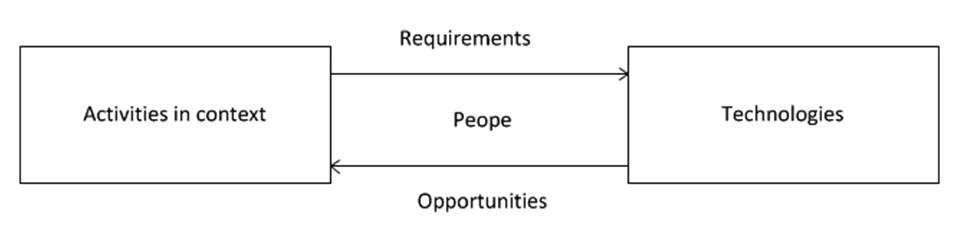
\includegraphics[width=0.70\textwidth]{img/PACT.png}
	\caption{PACT model}
	\label{fig:PACT}
\end{figure}

\subsubsection{People - the kindergarten teacher}
Kristine is in her thirties and is a fully educated pedagogue. Beyond this she has taken several degrees and courses focusing on the needs of children with mental handicaps, all resulting in her now working at Birken.

She takes care of a few selected children of those attached to the kindergarten, an activity that requires almost constant supervision while they are present. Kristine and her colleagues yearn for solutions that can ease and improve their daily work, particularly within the domains of communication with the children and their parents. Very notably, the time required to add a picture to an entry in the child's contact book is so severe that she cannot do it very often, a hindrance that bothers her. She would very much like to be able to attach an image to the book every day to improve the dialogue between child and parent.

\subsubsection{Activities}
\begin{itemize}
	\item Each day an entry is written in the contact book of every child, detailing the highlights of the day. It may be a single sentence or a paragraph with a picture of the child engaging in an activity. This is done by the kindergarten teachers, but entries may be commented on or entered a new by parents with any important thoughts.
	\item If a picture is to be added, first the picture is taken with a digital camera, imported into a desktop computer, then cropped, resized or rotated as necessary. Finally, the image is printed onto paper, cut out and glued into the contact book.
	\item Child and parent will sit down with the book, using the image in the book (if present) as a starting point for dialogue about the day, continuing through available pictograms.
\end{itemize}

\subsubsection{Contexts}
There are three contexts based on the three activities, two of them sufficiently similar to be written as one.
\begin{itemize}
	\item When compiling an entry in the contact book, the kindergarten teacher or guardian will sit by themselves, the child occupied either with their own devices or the supervision of someone else. 
	\item When discussing the entry in the book, however, child and parent are together.
\end{itemize}

\subsubsection{Technology}
Currently, two hardware technologies are in play: A digital camera, and a personal computer.
An image manipulation suite is used to edit the photographs. Possibly,  a Windows pre-installed application like MS Paint.

\subsubsection{Conclusion}
Even at a glance, several possible improvements can be suggested that make use of IT. Central are the notions of digitizing the contact book and easing the creation of images by using a mobile device with image manipulation software capable of the actions necessary.

\subsection{Problem formulation}
In our project we want to make it possible to use a computer to change the mobile device settings, but our primary focus will be to make a digitized version of the contact book so that kindergarten teachers and parents, easily and quickly, can exchange information. The kindergarten teachers will then be able to write and send a summary of the child's activities including pictures of the involved activities to the parents. This is the base for our system definition.